\documentclass{aiaa-tc}

%\usepackage[margin=1.0in]{geometry}
\usepackage{fullpage}
\usepackage{graphicx}
\usepackage{bm} %required for bold in math mode for greek symbols
\usepackage{amsmath} %for bmatrix
\usepackage{amsfonts} %for math script font
\usepackage{url} %for website citations

\usepackage[space]{grffile} %for filepaths with spaces

%define degree symbol:
\newcommand{\degree}{\ensuremath{^\circ}}

\newcommand{\fr}[1]{$#1^+$} %command to write a reference frame
\newcommand{\br}[2]{[#1]_{#2}} %bracket operator with subscript
\newcommand{\tvect}[3]{\begin{bmatrix}#1\\#2\\#3\end{bmatrix}}% 3 x 1 vector
\newcommand{\tvecth}[3]{\begin{bmatrix}#1&#2&#3\end{bmatrix}}% 1 x 3 vector
\newcommand{\B}[1]{\textbf{#1}} %bold for regular vectors
\newcommand{\U}[1]{\hat{\textbf{#1}}} %hats and bold for unit vectors
\newcommand{\BG}[1]{{\bm #1}}           % for vectors using greek letters
\newcommand{\ddt}[1]{\frac{d#1}{dt}} %for time derivatives
\newcommand{\kron}{\otimes} %redefines \kron to produce kronecker product symbol, for convenience

\title{Summary of 2D cooperative estimation \\ \large{With range and bearing to landmarks and to other agents}}
\author{Tim Woodbury}

\let\endtitlepage\relax %surpress line break after title page

\begin{document}

\maketitle

\section{Theoretical background and math}

\subsection{ EKF formulation of relative range measurements }

For agent $i$ to utilize relative range and/or bearing measurements to agent $j$, agent $i$ must either have an estimate of agent $j$'s position and velocity, or must have access to landmark measurements made by agent $j$. In the absence of either, agent $i$ must approximate $j$'s position as stationary, which inherently makes interagent measurements more uncertain than landmark measurements (assuming sensor accuracy is similar in both cases). When landmark ranges are not available, this approach could still provide some benefit if interagent range is measured. However, if $i$ has an estimate of $j$'s state, $i$ can do substantially better. This estimate could be provided directly from agent $j$'s onboard estimation, in which case we are essentially considering the case of a centralized filter; alternately, $j$ can provide IMU data to $i$. If IMU data from $j$ are available, then $i$ can propagate a model of both vehicles. There are many considerations with regard to sharing IMU data; required data rates for adequate estimation, bandwidth, potential range limitations, etc. Initially, we assume that extra-vehicle IMU measurements are not available. Therefore, we confine ourselves to the second case outlined above, where $i$ has access to landmark measurements made by $j$. In this case, the relationship between $j$'s measurements and $i$'s expectation of these measurements can be determined by leveraging interagent measurements, although the relationship is highly nonlinear.

First, some notation is established. $\rho$ and $\theta$ are adopted to indicate range and bearing, and bearing is measured relative to a vehicle's body 1-axis. A measurement of object $j$ relative to object $i$, e.g. the range measurement of object $j$ made by $i$, is denoted as $\rho_{ji}$. Bearing can only be defined in terms of an agent or other entity that has a definite heading $\psi$ in inertial space. For a generic landmark $k$ and two agents $i$ and $j$, we can define relationships between $j$'s measurements $\rho_{kj}$ and $\theta_{kj}$ and $i$'s expectation:

\begin{align}
\B{r}_{ji} = \B{r}_{j} - \B{r}_{i} \\
\br{\B{r}_{j}}{b} \equiv \begin{bmatrix}
r_{jx} \\
r_{jy}
\end{bmatrix} \\
\phi_{ji} \equiv \theta_{ji} + \psi_i \\
\br{r_{ji}}{b} = \rho_{ji}\begin{bmatrix}
\cos{\phi_{ji}}\\
\sin{\phi_{ji}}
\end{bmatrix}\\
\tan{\phi_{kj}} = \frac{r_{ky}-r_{jy}}{r_{kx}-r_{jx}}\\
\theta_{kj} = \arctan{\frac{r_{ky}-r_{jy}}{r_{kx}-r_{jx}}} - \psi_j\\
 = \arctan{ \frac{(r_{ky}-r_{iy}) - (r_{jy}-r_{iy})}{(r_{kx}-r_{ix}) - (r_{jx}-r_{ix})} } - \psi_j \\
 = \arctan{ \frac{(r_{ky}-r_{iy}) - \rho_{ji}\sin{ (\theta_{ji} + \psi_i )}}{(r_{kx}-r_{ix}) - \rho_{ji}\cos{(\theta_{ji} + \psi_i )}} } - \psi_j
 \label{eq:thetakj}
\end{align}

In Eq. \ref{eq:thetakj}, the bearing measurement $\theta_{kj}$ of landmark $k$ by agent $j$ has been written in terms of variables that are known by agent $i$. $\B{r}_{k}$ will be either known (as assumed here) or estimated, as assumed in later work. $\B{r}_i$ and $\psi_i$ are estimated internal agent states. $\rho_{ji}$ and $\theta_{ji}$ are measured directly. Finally, it should be noted that an estimate of agent $j$'s heading, $\psi_j$, is also required. For now, it is assumed that this estimate is provided directly from agent $j$ to $i$.

When landmark ranges are available, an expression also exists for landmark range from agent $j$ to $k$ in terms of variables known to agent $i$:

\begin{equation}
\rho_{kj} = \sqrt{ (r_{kx}-r_{ix}-\rho_{ji}\cos{\phi_{ji}})^2 + (r_{ky}-r_{iy}-\rho_{ji}\sin{\phi_{ji}})^2 }
\label{eq:rhokj}
\end{equation}

%When landmark ranges are available, we can also find an expression for interagent range in terms of estimated, known, and measured quantities, in Eq. \ref{eq:rhoji}:
%\begin{align}
%\rho_{ji} = \| \B{r}_j \| \| \B{r}_i \| \\
%= \| -\B{r}_{kj} + \B{r}_k - \B{r}_i \| \\
%= \| -\rho_{kj} \begin{bmatrix}
%\cos{\phi_{kj}} \\
%\sin{\phi_{kj}}
%\end{bmatrix} + \B{r}_k - \B{r}_i \| \\
%=\ \sqrt{ \rho_{kj}^2 - 2\rho_{kj} ((r_{kx}-r_{ix})\cos{\phi_{kj}} + (r_{ky}-r_{iy})\sin{\phi_{kj}}) + (r_{kx}-r_{ix})^2 + (r_{ky}-r_{iy})^2} \label{eq:rhoji}
%\end{align}
%In the case where landmark-to-agent ranges are not measured, then Eq. \ref{eq:rhoji} cannot be used by agent $i$ unless agent $j$ provides its estimate of $\rho_kj$.

We turn now to the derivation of appropriate noise terms associated with Eqs. \ref{eq:thetakj} and \ref{eq:rhokj}. Every term in these expressions, with the possible exception of $\B{r}_k$, has some associated uncertainty. To first order, the variance $R_y$ associated with a nonlinear function $\B{y} = f(\B{x}), \B{x} \sim N(0,R_x)$ can be written in terms of the Jacobian of \B{y} with respect to each random variable in \B{x}, J, and the associated covariance matrix $R_x$:

\begin{equation}
R_y = JR_xJ^T \\
J \equiv \begin{bmatrix}
\frac{ \partial y_1 }{ \partial \B{x} }^T \\
\frac{ \partial y_2 }{ \partial \B{x} }^T \\
\vdots \\
\frac{ \partial y_m }{ \partial \B{x} }^T \\
\end{bmatrix}
\label{eq:covTransf}
\end{equation}

For completeness, partial derivatives are enumerated below:

\begin{align}
\frac{ \partial \theta_{kj} }{ \partial r_{ix} } = 
\frac{ r_{ky}-r_{iy} - \rho_{ji}\sin{\phi_{ji}} }{ (r_{kx}-r_{ix} - \rho_{ji}\cos{\phi_{ji}})^2 + (r_{ky}-r_{iy} - \rho_{ji}\sin{\phi_{ji}})^2 } \\
\frac{ \partial \theta_{kj} }{ \partial r_{iy} } = 
-\frac{ r_{kx}-r_{ix} - \rho_{ji}\cos{\phi_{ji}} }{ (r_{kx}-r_{ix} - \rho_{ji}\cos{\phi_{ji}})^2 + (r_{ky}-r_{iy} - \rho_{ji}\sin{\phi_{ji}})^2 } \\
\frac{ \partial \theta_{kj} }{ \partial \psi_{i} } = 
\frac{ \rho_{ji}^2 - \rho_{ji}((r_{kx}-r_{ix})\cos{\phi_{ji}}+(r_{ky}-r_{iy})\sin{\phi_{ji}}) }{ (r_{kx}-r_{ix} - \rho_{ji}\cos{\phi_{ji}})^2 + (r_{ky}-r_{iy} - \rho_{ji}\sin{\phi_{ji}})^2 } \\
\frac{ \partial \theta_{kj} }{ \partial \rho_{ji} } = 
\frac{ -(r_{kx}-r_{ix})\sin{\phi_{ji}} + (r_{ky}-r_{iy})\cos{\phi_{ji}} }{ (r_{kx}-r_{ix} - \rho_{ji}\cos{\phi_{ji}})^2 + (r_{ky}-r_{iy} - \rho_{ji}\sin{\phi_{ji}})^2 } \\
\frac{ \partial \theta_{kj} }{ \partial \theta_{ji} } = 
\frac{ \rho_{ji}^2 - \rho_{ji}((r_{kx}-r_{ix})\cos{\phi_{ji}}+(r_{ky}-r_{iy})\sin{\phi_{ji}}) }{ (r_{kx}-r_{ix} - \rho_{ji}\cos{\phi_{ji}})^2 + (r_{ky}-r_{iy} - \rho_{ji}\sin{\phi_{ji}})^2 } \\
\frac{ \partial \theta_{kj} }{ \partial \psi_{j} } = -1
\end{align}

The variables $\rho_{ji}$ and $\theta_{ji}$ are independent measurements and have no associated covariance with other variables. It is assumed that the available estimate of $\phi_j$, the other agent's heading, is also independent of the other terms in the expression, and has variance equal to agent $j$'s current associated variance; in truth, there is some codependence between the estimated states of agents $i$ and $j$ due to sharing of measurements, but this is assumed to be a higher-order term than the others present. Therefore, the covariace matrix $R_x$ is diagonal except for the covariance between agent $i$'s estimates $r_{ix}$, $r_{iy}$, and $\psi_i$:

\begin{equation}
R_x = \begin{bmatrix}
P_{k,i}^{-}(r_{ix},r_{iy},\psi_i) & \B{0}_{3\times 3} \\
\B{0}_{3\times 3} & \mathrm{diag}(\sigma_{\rho_{ji}}^2,\sigma_{\theta_{ji}}^2,P_{k,j}^{-}(\psi_j) )
\end{bmatrix}
\end{equation}

Eq. \ref{eq:covTransf} yields, in general, a fully populated $6\times 6$ covariance matrix $R_y$ for the expectation of the measurement. The measurement itself has an expected variance based on sensor properties; the total variance is assumed to be the sum of the sensor-based variance and the additional variance computed from Eq. \ref{eq:covTransf}. If $\rho_{kj}$ is available, it is incorporated by appending additional rows to the Jacobian. Its partials are listed below:

\begin{align}
\frac{ \partial \rho_{kj} }{ \partial r_{ix} } = 
-\frac{ r_{kx}-r_{ix}-\rho_{ji}\cos{\phi_{ji}} }{\rho_{kj}} \\
\frac{ \partial \rho_{kj} }{ \partial r_{iy} } = 
-\frac{ r_{ky}-r_{iy}-\rho_{ji}\sin{\phi_{ji}} }{\rho_{kj}} \\
\frac{ \partial \rho_{kj} }{ \partial \psi_{i} } = 
\frac{ -\rho_{ji}\cos{\phi_{ji}}(r_{ky}-r_{iy}-\rho_{ji}\sin{\phi_{ji}}) + \rho_{ji}\sin{\phi_{ji}}(r_{kx}-r_{ix}-\rho_{ji}\cos{\phi_{ji}}) }{\rho_{kj}} \\
\frac{ \partial \rho_{kj} }{ \partial \rho_{ji} } = 
\frac{ -\cos{\phi_{ji}}(r_{kx}-r_{ix}-\rho_{ji}\cos{\phi_{ji}}) - \sin{\phi_{ji}}(r_{ky}-r_{iy}-\rho_{ji}\sin{\phi_{ji}}) }{\rho_{kj}} \\
\frac{ \partial \rho_{kj} }{ \partial \theta_{ji} } = \frac{ -\rho_{ji}\cos{\phi_{ji}}(r_{ky}-r_{iy}-\rho_{ji}\sin{\phi_{ji}}) + \rho_{ji}\sin{\phi_{ji}}(r_{kx}-r_{ix}-\rho_{ji}\cos{\phi_{ji}}) }{\rho_{kj}} \\
\frac{\partial \rho_{kj}}{\partial \psi_j} = 0
\end{align}

Finally, note that when landmark positions are unknown, i.e. $\B{r}_k$ is an estimated state as well, the partial derivatives with respect to its components are simply the negative of the partials with respect to $\B{r}_i$. With this knowledge, the formulation outlined for the case with range, bearing, and known landmarks should be readily extensible to unknown landmarks without all of the measurements.

\section{Simulation results}

\subsection{Good relative measurements, poor landmark measurements}

The measurement variances for this case are:

\begin{eqnarray}
\sigma^2_{range,landmark} = 100 \\
\sigma^2_{bearing,landmark} = .01\\
\sigma^2_{range,agent} = 1 \\
\sigma^2_{bearing,agent} = .0001\\
R_{imu} = \mathrm{diag}\tvecth{.25}{.25}{.01}
\end{eqnarray}

Three landmarks and two agents are considered. Essentially, the low relative uncertainty effectively permits each agent to access twice as many landmark measurements with no additional uncertainty.

\begin{figure}[p]
\centering
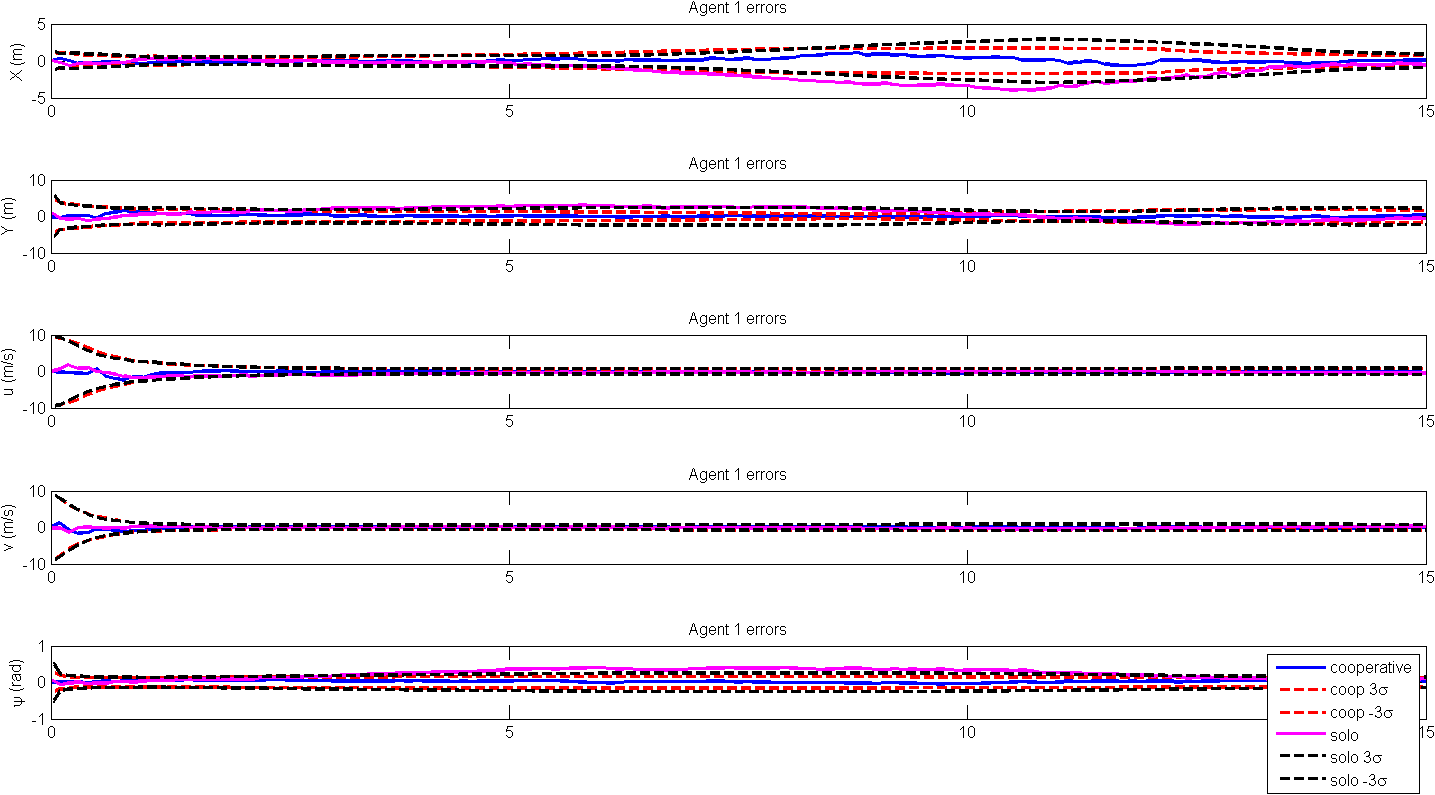
\includegraphics[height=0.4\textheight]{../good_relative_agent1.png}
\caption{Agent 1 estimate error histories with estimated variance 3$\sigma$ bounds for individual and cooperative estimation cases. $\sigma^2_{range,landmark} = 100,\sigma^2_{bearing,landmark} = .01,\sigma^2_{range,agent} = 1,\sigma^2_{bearing,agent} = .0001$}
\label{fig:good_relative_agent1}
\end{figure}

\begin{figure}[p]
\centering
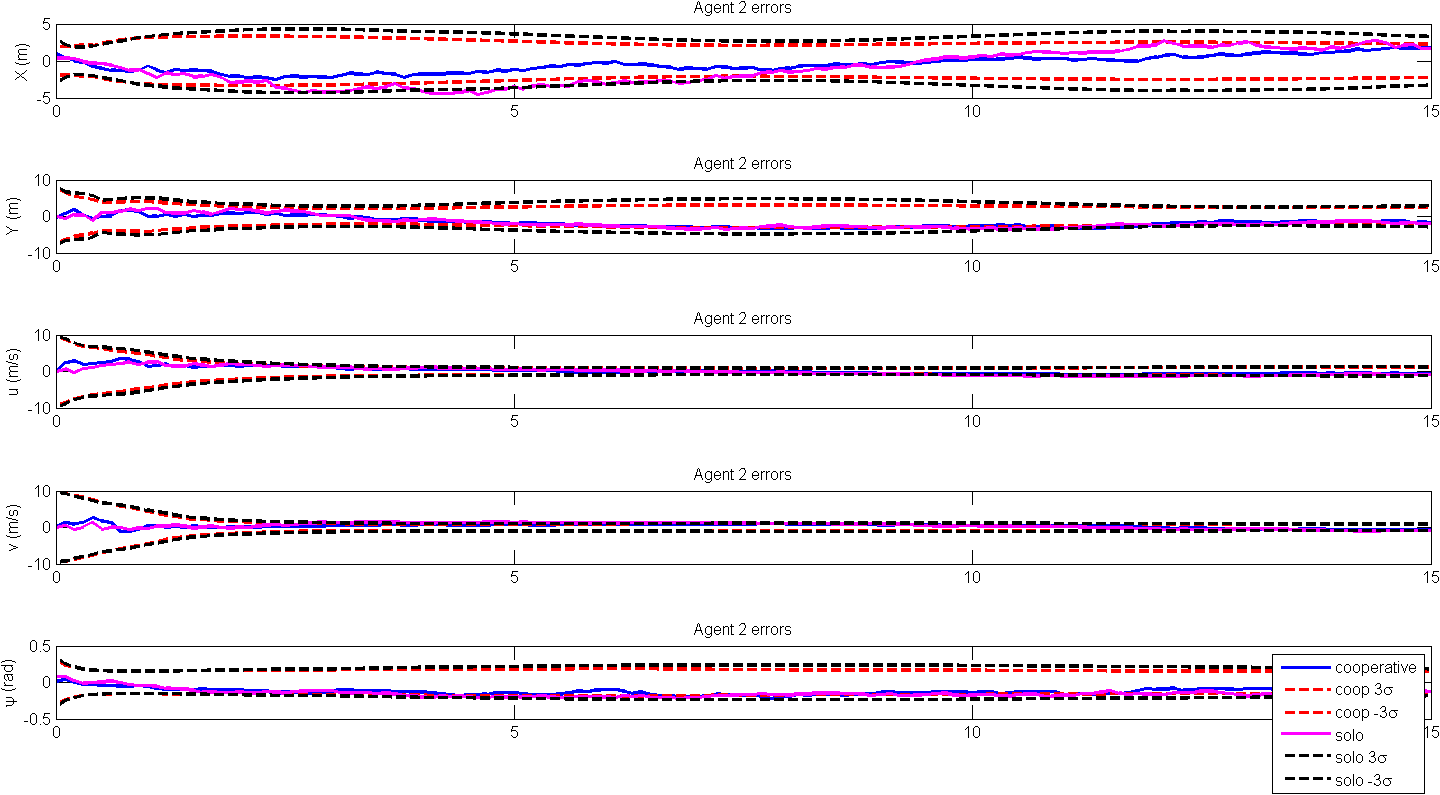
\includegraphics[height=0.4\textheight]{../good_relative_agent2.png}
\caption{Agent 2 estimate error histories with estimated variance 3$\sigma$ bounds for individual and cooperative estimation cases. $\sigma^2_{range,landmark} = 100,\sigma^2_{bearing,landmark} = .01,\sigma^2_{range,agent} = 1,\sigma^2_{bearing,agent} = .0001$}
\label{fig:good_relative_agent2}
\end{figure}

\subsection{Good landmark measurements, poor relative measurements}

The measurement variances for this case are:

\begin{eqnarray}
\sigma^2_{range,landmark} = 10 \\
\sigma^2_{bearing,landmark} = .001\\
\sigma^2_{range,agent} = 100 \\
\sigma^2_{bearing,agent} = .01\\
R_{imu} = \mathrm{diag}\tvecth{.25}{.25}{.01}
\end{eqnarray}

120 seconds of simulation were conducted. Graphically, there is little difference in the appearance of the convergence or long-term error bound of the two cases at this noise level. Mean squared error over the full simulation is used to compare the two cases. As seen in Table \ref{tab:good_landmark}, there is little difference in the MSE between the two cases; some values are lower for the cooperative case and some values are better for the individual case. This result is typical of the case where the relative measurements are less accurate than the landmark measurements; the uncertainty associated with the additional measurements is large enough that there is little gained in terms of MSE or convergence time.

\begin{table}
\centering
\begin{tabular}{ccccccc}
Case & Agent & $MSE_X$ & $MSE_Y$ & $MSE_u$ & $MSE_v$ & $MSE_\psi$\\ 
Cooperative & 1 &0.02747 &0.05879 &0.02255 &0.03492 &0.0007725\\ 
Cooperative & 2 &0.01279 &0.03048 &0.01589 &0.01604 &0.0003827\\ 
Individual & 1 &0.0194 &0.03475 &0.02847 &0.01924 &0.0005208\\ 
Individual & 2 &0.01735 &0.04088 &0.01671 &0.02335 &0.0003919\\
\end{tabular}
\caption{Mean squared estimate errors with $\sigma^2_{range,landmark} = 10, \sigma^2_{bearing,landmark} = .001,\sigma^2_{range,agent} = 100, \sigma^2_{bearing,agent} = .01,R_{imu} = \mathrm{diag}\tvecth{.25}{.25}{.01}$.}
\label{tab:good_landmark}
\end{table}

\end{document}
